% Adapted from LLNCS.DEM Springer-Verlag for LNCS, version 2.3 for LaTeX2e
\documentclass{llncs}
\usepackage{czt}  %% for the Standard Z specification macros
\usepackage{graphics}
%
\begin{document}
\pagestyle{headings}  % switches on printing of running heads
%
\title{Testing a Z Specification of Posix}
\titlerunning{Testing a Z Spec of Posix}  % abbreviated title (for running head)
%                                     also used for the TOC unless
%                                     \toctitle is used
%
\author{Mark Utting\inst{1} \and Petra Malik\inst{2}}
%
\authorrunning{Utting and Malik}   % abbreviated author list (for running head)
%
%%%% list of authors for the TOC (use if author list has to be modified)
%\tocauthor{Mark Utting, Petra Malik}
%
\institute{Department of Computer Science, The University of Waikato, NZ\\
\email{marku@cs.waikato.ac.nz},\\
% WWW home page: \texttt{http://www.cs.waikato.ac.nz/\homedir marku}
\and
Faculty of Engineering,
Victoria University of Wellington, NZ
\email{petra.malik@mcs.vuw.ac.nz}
}

\maketitle              % typeset the title of the contribution

\begin{abstract}
We refactor Morgan and Suffrin's original Z specification of the
Posix file system, to break it into Z sections and make it conform
to the Z Standard.  We develop a simple framework for testing Z
specifications, and use this framework to test the first few levels
of the specification.  The tests are written in standard Z, and are
executable by the CZT animator, ZLive.
\end{abstract}

%%%%%%%%%%%%%%%%%%%%%%%%%%%%%%%%%%%%%%%%%%%%%%%%%%%%%%%%%%%%%%%%%%%%%%
\section{Introduction}
%%%%%%%%%%%%%%%%%%%%%%%%%%%%%%%%%%%%%%%%%%%%%%%%%%%%%%%%%%%%%%%%%%%%%%

In~\cite{Hoa03}, Hoare proposes a grand challenge for computer
science---a verifying compiler---and inspired researchers from all
over the world to work jointly towards this ambitous goal.  The
verified software repository~\cite{BicHoaWoo06} is a means to record
and coordinate these efforts.  The repository contains an evolving
collection of tools related to software verification as well as case
studies.

The pilot case studies for the verified software repository are
carefully chosen.  They are sufficiently complex to be challenging and
of industrial relevance but small enough to be completed within a few
years.  They provide examples of specified and verified code and can
be used as benchmarks to exercise and test current and future
verification tools.

The Mondex case study was tackled as a first challenge in 2006.
Several teams using a variety of techniques and tools were working on
a fully automated proof of the Mondex smart-card banking application.
A verifiable filesystem has been proposed~\cite{JosHol07} as another
mini challenge.  An initial small subset of POSIX was chosen and
participants of the ABZ 2008 conference were challenged to contribute
to this project.

This paper discusses a simple framework for testing Z specifications.
The framework has been used to test the first few levels of a
refactored version of Morgan and Suffrin's Z specification of
the Posix file system~\cite{MorSufTOSE84}.  TODO: ...



%%%%%%%%%%%%%%%%%%%%%%%%%%%%%%%%%%%%%%%%%%%%%%%%%%%%%%%%%%%%%%%%%%%%%%
\section{Posix Standardized}
%%%%%%%%%%%%%%%%%%%%%%%%%%%%%%%%%%%%%%%%%%%%%%%%%%%%%%%%%%%%%%%%%%%%%%

In this section, we describe the refactored Posix specification.
The main change was to break up the original specification into
sections.  Figure~\ref{fig:sects} shows the structure of the
resulting Z sections, using a notation similar to a UML class diagram.
Each box represents a Z section, and the three parts within each box
show the name of the section, the main variables within the state
schema of that definition, and the names of its operation schemas
(we omit Init schemas and auxiliary schemas).

As well as breaking the specification into sections, we made several other
changes.  TODO: describe the other changes we made.


\begin{figure}[htbp]
\newcommand{\DIVIDER}{\vspace{0.5ex} \hrule \vspace{1ex}}
\newcommand{\FATDIVIDER}{\vspace{1ex} \hrule \vspace{1.5ex}}
\newcommand{\SECTNAME}[2]{\hfil\hfil\hfil\textbf{#1}\hfil\emph{(#2)}}
  \centering
  \setlength{\unitlength}{1cm}
  \begin{picture}(10,20)
%
  \put(1,18){\framebox(8,1){\parbox{6cm}{
        \hfil \textbf{standard\_toolkit} \hfil
    }}}
  \put(5,17){\vector(0,1){1}}
  \put(1,15){\framebox(8,2){\parbox{8cm}{
        \SECTNAME{DS}{Data System}
        \DIVIDER
        ~$FILE == \seq BYTE$ \\ \hbox{}
        ~$file : FILE$
        \DIVIDER
        $~readFILE, writeFILE$
    }}}
  \put(5,14){\vector(0,1){1}}
  \put(1,12){\framebox(8,2){\parbox{8cm}{
        \SECTNAME{SS}{Storage System}
        \FATDIVIDER
        ~$fstore : FID \pfun FILE$
        \FATDIVIDER
        $~createSS, destroySS, readSS, writeSS$
    }}}
  \put(5,11){\vector(0,1){1}}
  \put(1,9){\framebox(8,2){\parbox{8cm}{
        \SECTNAME{CS}{Channel System}
        \FATDIVIDER
        ~$cstore : CID \pfun CHAN$
        \FATDIVIDER
        $~openCS, closeCS$
    }}}
  \put(5,8){\vector(0,1){1}}
  \put(1,6){\framebox(8,2){\parbox{8cm}{
        \SECTNAME{AS}{Access System}
        \FATDIVIDER
        ~$SS; CS$
        \FATDIVIDER
        $~readAS, writeAS, seekAS$
    }}}
  \put(5,5){\vector(0,1){1}}
  \put(1,3){\framebox(8,2){\parbox{8cm}{
        \SECTNAME{NS}{Name System}
        \FATDIVIDER
        ~$nstore : NAME \pfun FID$
        \FATDIVIDER
        $~createNS, lookupNS, destroyNS, lsNS$
    }}}
  \put(5,2){\vector(0,1){1}}
  \put(1,0){\framebox(8,2){\parbox{8cm}{
        \SECTNAME{FS}{File System}
        \DIVIDER
        ~$SS; CS; NS; usedfids : \power FID$
        \DIVIDER
        $~createFS, openFS, readFS, writeFS, closeFS,$ \\
        \hbox{}$~unlinkFS0, destroyFS, linkFS, moveFS$
    }}}

  \end{picture}
  \caption{Overview of Z Sections in the Posix Specification}
  \label{fig:sects}
\end{figure}

\input{ds.zed}


%%%%%%%%%%%%%%%%%%%%%%%%%%%%%%%%%%%%%%%%%%%%%%%%%%%%%%%%%%%%%%%%%%%%%%
\section{How to Test a Z Specification}
%%%%%%%%%%%%%%%%%%%%%%%%%%%%%%%%%%%%%%%%%%%%%%%%%%%%%%%%%%%%%%%%%%%%%%

This section introduces a simple framework for expressing tests
of a Z specification.  We assume that the specification is written in the
common Z \emph{sequential} style, with a state schema, an initialisation
schema, several operation schemas, as well as various auxiliary definitions
and schemas.

The first question that must be asked is why we do not use an existing
testing framework for Z, such as the Test Template Framework
(TTF)~\cite{Stocks93,carrington94} or Heirons' Z-to-FSM
approach~\cite{hierons97}.  The difference is that these all aim at
generating tests \emph{from} a Z specification, in order to test some
implementation of that specification.  But in this paper, we want to design
some tests that actually test the Z specification itself.  So the goal of
those approaches is \emph{verification} (of some implementation), whereas
our goal is \emph{validation} (of the Z specification).  This results in
quite a different style of testing.  

One difference is that when testing an implementation, we can control its
inputs but not its outputs, whereas when testing a Z specification we can
ask arbitrary questions about inputs or outputs.  So when validating a Z
specification, we can use a richer variety of tests.  Another difference is
that when validating a specification, we want to design both positive
tests, which test that a given behaviour is allowed by the specification,
and negative tests, which test that a given behaviour is not allowed by the
specification.  In contrast, when testing an implementation of the
specification, we use only positive tests, because refinement means that
the implementation is free to add behaviour that is outside the
precondition of the specification.

To illustrate our testing framework, we shall use a simple example
specification given by the following specification, which defines
the shape shown in Figure~\ref{fig:wedge}.
Our tests will be written using standard Z conjecture paragraphs,
so that they can be checked by theorem provers or by the ZLive
animator.  We use one or more Z sections for the specification,
and then group the tests into separate Z sections that have the
specification as a parent.

\begin{figure}[htbp]
  \centering
  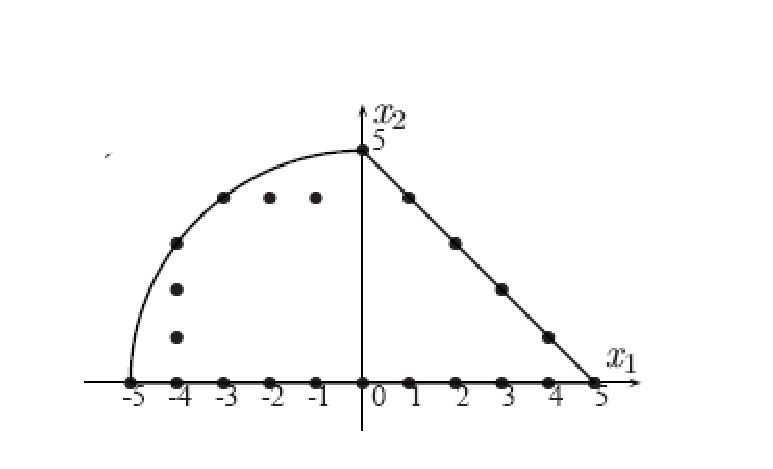
\includegraphics{wedge}
  \caption{A graph of the solutions to the Wedge schema}
  \label{fig:wedge}
\end{figure}

\begin{zsection}
  \SECTION wedge \parents standard\_toolkit
\end{zsection}
\begin{zed}
  State == [n: \negate 10 \upto 10] \\
  Wedge == [\Delta State | n*n + n'*n' \leq 25; n + n' \leq 5; 0 \leq n']
\end{zed}

\subsection{Positive Tests}

The first kind of testing we want to do is positive tests to check that an
operation has a desired input-output behaviour.  When specifying
tests, it is important to specify the expected output values as well as the
input values, so we write all the inputs and output values as a Z binding
and use a membership test.  Here are two examples that test the
non-deterministic output behaviour of Wedge when the input $x=0$.
Since 2007, the Z standard requires conjectures to be written within
a \LaTeX\ \emph{theorem} environment, and allows each conjecture to be
given a name.  Our naming convention for tests is typically to use the name
of the operation being tested, followed by some information about the input
and output values that are being tested.

\begin{zsection}
  \SECTION wedgeTests \parents wedge
\end{zsection}

\begin{theorem}{Wedge0Min}
\vdash? ~~ \lblot n==0, n'==0 \rblot \in Wedge
\end{theorem}

\begin{theorem}{Wedge0Max}
\vdash? ~~ \lblot n==0, n'==5 \rblot \in Wedge
\end{theorem}

Alternatively, we may prefer to group a set of tests together, and test
them all in one conjecture.  We can do this by naming the test tuples, and
testing them all using a subset conjecture.

\begin{zed}
  Wedge0Min == \lblot n==0, n'==0 \rblot \\
  Wedge0Max == \lblot n==0, n'==5 \rblot
\end{zed}

\begin{theorem}{WedgePos}
  \vdash? ~~ \{Wedge0Min, Wedge0Max\} \subseteq Wedge
\end{theorem}


\subsection{Negative Tests}

It is also useful to perform \emph{negative} tests to validate an
operation.  For example, we may want to check that an input value is
outside the precondition of the operation, or check that a certain output
can never be produced by the operation.  The idea is to validate the
specification by showing that its behaviour is squeezed in between the set
of positive tests and the set of negative tests.  The more positive and
negative tests that we design, the more sure we can be that we have
specified the desired behaviour, rather than allowing too many or too few
behaviours.

We can write negative tests using a negated membership test ($test \notin
Op$) or, equivalently, test that the tuple is a member of the negated
schema ($test \in \lnot Op$).
Our conjecture naming convention is the same as for positive tests, but
we prefix the name with $Not$ to indicate that it is a negative tests.

\begin{zsection}
  \SECTION notWedgeTests \parents wedge
\end{zsection}

\begin{theorem}{NotWedge0Neg}
\vdash? ~~ \lblot n==0, n'==\negate 1 \rblot \notin Wedge
\end{theorem}

\begin{theorem}{NotWedge06}
\vdash? ~~ \lblot n==0, n'==6 \rblot \in \lnot Wedge
\end{theorem}

We can also test just the precondition of the operation.
%% Note: ZLive cannot evaluate this if the type of x is any integer
%% because it requires enumerating pre Wedge, and then there is no
%% lower bound on $n'$.
\begin{theorem}{NotWedgePre6}
\vdash? ~~ \lblot n==6 \rblot \notin \pre Wedge
\end{theorem}

As we did for positive tests, we may also combine several negative tests
into a group.  In this case, our conjecture may be written as $tests
\subseteq \lnot Op$, or equivalently we may check that the intersection of
the negative test suite and the operation is empty, $tests \land Op =
\emptyset$.  The latter style is often more convenient, since it allows us
to write $tests$ using schema notation, and to omit variables that we are
not interested in (because the schema conjunction will expand the type of
$tests$ to match the type of $Op$).  For example, the following two negative
test suites check that 6 can never be an input for $Wedge$, and that 6 can
never be an output of $Wedge$.

\begin{theorem}{NotWedgeIn6}
\vdash? ~~ ([State | n=6] \land Wedge) = \emptyset
\end{theorem}

\begin{theorem}{NotWedgeOut6}
\vdash? ~~ ([State~' | n'=6] \land Wedge) = \emptyset
\end{theorem}

It is sometimes convenient to write these kinds of negative test values
\emph{within} the operation schema (e.g., $[Wedge | x=6] = \emptyset$),
which can make the tests even more concise.


\subsection{Promoting Tests}

A heavily-used pattern in the Posix Z specification is the use of
\emph{promotion} to lift the operations of one data type up to work on a
more complex data type.  It is useful to be able to promote the tests
of those operations as well.  To illustrate an elegant way of doing this,
we shall promote the $Wedge$ tests up to the following function space:

\begin{zsection}
  \SECTION manyStates \parents wedge
\end{zsection}

\begin{schema}{ManyStates}
  states : \nat \fun \num
\end{schema}

\begin{schema}{\Phi ManyStates}
  \Delta State \\
  \Delta ManyStates \\
  curr? : \nat
\where
  (curr? \mapsto n) \in states \\
  states' = states \oplus \{curr? \mapsto n'\}
\end{schema}

We promote the $Wedge$ operation up to the $ManyStates$ level simply by
conjoining $Wedge$ with the \emph{framing schema} $\Phi ManyStates$.
The effect is to apply the $Wedge$ operation to just the $curr?$ element of
the $states$ function. 

\begin{zed}
  ManyWedge == \Phi ManyStates \land Wedge
\end{zed}


We use the same framing schema to promote the tests.  But to ensure that
all inputs of the promoted operation are given, we use a specialised
version of the framing schema that also specifies an initial value
for the $states$ mapping and which $curr?$ input will be tested.

\begin{zsection}
  \SECTION manyStatesTest \parents manyStates, wedgeTests
\end{zsection}

\begin{zed}
  \Phi ManyStatesTest ==
    [\Phi ManyStates; curr? == 1 | states = \{0 \mapsto 3, 1 \mapsto n\}]
\end{zed}

%% NOTE: this fails if State contains x, because of a scoping
%% error in the unfolding or in the translation to FlatPreds.
%% Probably an 'x' in the ZLive preprocess rules gets accidentally
%% bound to the 'x' from the State schema.
\begin{theorem}{ManyWedgePos}
  \vdash? ~~ (\{Wedge0Min, Wedge0Max\} \land \Phi ManyStatesTest)
      \subseteq ManyWedge
\end{theorem}

In fact, this style of promoted test theorem will always be true,
because for any test suite $OpTests$ of an operation $Op$,
and any promoted operation defined as $Op_P == Op \land \Phi P$,
it is true that:
\[
   (OpTests \in Op) \land (\Phi PTests \subseteq \Phi P)
   \implies (OpTests \land \Phi PTests \subseteq Op_P)
\]

\textbf{Proof:} follows from the monotonicity of $\subseteq$ and schema
conjunction.

However, there is a possibility that some of the promoted tests
will be inconsistent with the framing schema (either $\Phi P$ or $\Phi
PTests$), which would mean that the set $OpTests \land \Phi PTests$
would be empty or smaller than our original set of tests $Optests$.
If we want to check that all of the original tests can be promoted without
being lost, we can check the conjecture 
$(OpTests \land \Phi PTests) = Optests$.

If this is not true, we may want to check each test vector $v \in Optests$
separately.  We can define the promoted vector as 
$pv == (\mu \Phi PTests | \theta \{v\} = v)$.
Then we can test $pv \in Op_P$. 



%%%%%%%%%%%%%%%%%%%%%%%%%%%%%%%%%%%%%%%%%%%%%%%%%%%%%%%%%%%%%%%%%%%%%%
\section{The ZLive Animator}
%%%%%%%%%%%%%%%%%%%%%%%%%%%%%%%%%%%%%%%%%%%%%%%%%%%%%%%%%%%%%%%%%%%%%%

One of the tools available in the CZT system is the ZLive animator.
It is the successor to the Jaza animator for Z~\cite{utting:jaza}.

TODO: brief description of how ZLive works, and a trivial example.


%%%%%%%%%%%%%%%%%%%%%%%%%%%%%%%%%%%%%%%%%%%%%%%%%%%%%%%%%%%%%%%%%%%%%%
\section{Testing the DS Specification}
%%%%%%%%%%%%%%%%%%%%%%%%%%%%%%%%%%%%%%%%%%%%%%%%%%%%%%%%%%%%%%%%%%%%%%

\input{dstest.zed}


%%%%%%%%%%%%%%%%%%%%%%%%%%%%%%%%%%%%%%%%%%%%%%%%%%%%%%%%%%%%%%%%%%%%%%
\section{Testing the SS Specification}
%%%%%%%%%%%%%%%%%%%%%%%%%%%%%%%%%%%%%%%%%%%%%%%%%%%%%%%%%%%%%%%%%%%%%%

TODO: describe how we can use a framing schema to `promote' the DS tests
up to this level.  Give examples.


%%%%%%%%%%%%%%%%%%%%%%%%%%%%%%%%%%%%%%%%%%%%%%%%%%%%%%%%%%%%%%%%%%%%%%
\section{Conclusions}
%%%%%%%%%%%%%%%%%%%%%%%%%%%%%%%%%%%%%%%%%%%%%%%%%%%%%%%%%%%%%%%%%%%%%%

Testing is useful, especially when the execution of the tests can
be automated.

The refactored Z specification of Posix may be a useful starting point
for other researchers who want to work on refinement or proofs
about the Posix case study.  It is available from the CZT sourceforge
website...


%
% ---- Bibliography ----
%
\bibliographystyle{alpha}
\bibliography{posix}
%\begin{thebibliography}{5}
%
%\bibitem {clarke}
%TODO...
%\end{thebibliography}
\end{document}
